\section{Design and Implementation}
\label{sec:snarkprobe-design}

In this section, we introduce both the high level goals and concrete implementation decisions, tools, and techniques that allow us to realize \tool.  We start with the \ConstraintChecker and then discuss the various components of \SnarkFuzzer.  These two sub-tools can be used either in conjunction with each other, or separately, depending on what the developer wishes to check.

\subsection{\ConstraintChecker}
\label{subsec:snarkprobe-constraintchecker}

\parhead{Goals:} \emph{The \ConstraintChecker helps ensure that the realized proof is equivalent to a specified statement.  This also allows the \ConstraintChecker to find errors in flattening and/or gadget use.  It achieves this by comparing the equivalence of a user-specified proof statement and the compiled R1CS gates to ensure that the proof generated by the library represents the developer's specified statement\footnote{We note that we cannot do anything about the garbage-in-garbage-out problem (for example, the case where a developer implements a proof that misses a necessary case, such as omitting checking if a value is greater than 0).  We can just help determine if the specified statement and realized proof are likely equivalent.}.}

\parhead{Design.}%
The first step in generating a \zksnark proof is converting the desired proof statement equations into R1CS.  These R1CS gates should have the same domain, range, and output value as input statement equations.
To check this, we developed our \ConstraintChecker, which leverages an SMT solver and associated techniques to verify the equivalence of R1CS gates to the specified proof statement functions\footnote{We work around the general undecidability of function equality by operating in the more constrained setting (over the finite fields) and adding special rules for primary variables and auxiliary variables.}. To run the tool, the user only needs to write a short script to define the statement function, primary inputs, and auxiliary inputs in their zkSNARK proof, and everything else then happens automatically. \autoref{subfig:snarkprobe-workflow_cc} shows the key steps in the \ConstraintChecker, and we also provide an example in Listing \autoref{list:constraintchecker} of our \ConstraintChecker to show how a developer can run the tool. More examples can be found in our code. We note that our SMT solver could be replaced by any other techniques that allow one to check for function equality and fit the desired goals.
\definecolor{dkgreen}{rgb}{0,0.6,0}
\definecolor{gray}{rgb}{0.5,0.5,0.5}
\definecolor{mauve}{rgb}{0.58,0,0.82}

\lstset{
  frame=tb,
  language=Python,
  aboveskip=3mm,
  belowskip=3mm,
  showstringspaces=false,
  columns=flexible,
  basicstyle={\small\ttfamily},
  numbers=none,
  numberstyle=\tiny\color{gray},
  keywordstyle=\color{blue},
  commentstyle=\color{dkgreen},
  stringstyle=\color{mauve},
  breaklines=true,
  breakatwhitespace=false,
  breakindent=0pt,
  breakautoindent=false,
  xleftmargin=0pt,
  xrightmargin=0pt,
  framexleftmargin=5pt,
  framexrightmargin=0pt,
  tabsize=3
}

\begin{ZZlisting}[H]
\centering
\begin{adjustbox}{max width=\textwidth}
\begin{CenteredBox}
\begin{minipage}{0.96\textwidth}
\begin{lstlisting}
x = z3.Int("x")
## Indicate the public variables and private variables
allocate = ["x"]
variables = [x]
## Indicate the statement of a proof
statement = [x < 60]
## Provide the snark program to automatically extract the R1CS matrix
## Developer can also manually provide the R1CS matrix
path = os.path.join(currentdir, "range")
## Call the functions in ConstraintChecker to evaluate the correctness
fcmp = FunctionComparison(path)
fcmp.allocate(allocate)
fcmp.set_input_sizes(0)
fcmp.addVariables(variables)
fcmp.addStatement(statement)
fcmp.addGadget(gadget1.comparison_gadget("max")) ## Optional
fcmp.addRange(x, z3.And(x < 60))
fcmp.runComparisonTests()
\end{lstlisting}
\end{minipage}
\end{CenteredBox}
\end{adjustbox}
\caption{An example of \ConstraintChecker}
\label{list:constraintchecker}
\end{ZZlisting}
\parhead{Implementation.} The \ConstraintChecker contains two major components: the Circuit Extractor and a three-step equivalence check. We discuss these components in detail below. \autoref{pro:constraintchecker} presents the detailed procedure for each component. We discuss optimizations in \autoref{app:snarkprobe-constraintopt}.


\begin{protocol}[!htbp]
\centering
\begingroup
\makeatletter
\let\oldscriptsize\scriptsize
\renewcommand{\scriptsize}{\oldscriptsize\setlength{\baselineskip}{11.5pt}}
\makeatother

\setlength{\fboxsep}{6pt}
\setlength{\fboxrule}{0.35pt}

\vspace*{\fill}

\begin{adjustbox}{max width=\textwidth, max totalheight=0.92\textheight, keepaspectratio}
\begin{minipage}[t]{0.48\textwidth}

% ---------- (a) Parameters ----------
\fbox{%
\begin{minipage}[t]{0.95\textwidth}
\scriptsize
\raggedright
\setlength{\parindent}{0pt}
\setlength{\parskip}{0.35em}

\textbf{(a) Parameters.}

\begin{enumerate}[leftmargin=1.4em,itemsep=0.6em,topsep=0.25em,parsep=0.5em]
\item A set of statement equations $E_{1}$ in size $p$ where equation $e_{1}^{i} \in E_{1}$ and $i \in [1,p]$.
\item A set of equations $E_{2}$ converted from R1CS gates in size $q$ where $e_{2}^{i} \in E_{2}$ and $i \in [1,q]$.
\item $m$ private variables $x_{1}^{i}$ in $E_{1}$ where $i \in [1,m]$ and $n$ private variables $x_{2}^{i}$ in $E_{2}$ where $i \in [1,n]$ and $n \geq m$. A set of auxiliary input $v_{x}^{i}$.
\item $k$ public variables $y_{1}^{i}$ in $E_{1}$ and $k$ public variables $y_{2}^{i}$ in $E_{2}$ where $i \in [1,k]$. A set of primary input $v_{y}^{i}$.
\item A SMT Pro Solver $S$ and Optimizer $O$ with modulus $P$. $0 \leq x_{1} < P$, $0 \leq x_{2} < P$, $0 \leq y_{1} < P$, and $0 \leq y_{2} < P$ without optimization.

\vspace{0.5em}
\end{enumerate}
\end{minipage}%
}

\vspace{0.9em}

% ---------- SMT Solver ----------

\fbox{%
\begin{minipage}[t]{0.95\textwidth}
\scriptsize
\raggedright
\setlength{\parindent}{0pt}
\setlength{\parskip}{0.35em}

\textbf{SMT Solver:} The solver $S$ and optimizer $O$ are designed based on the Z3 theorem prover. Other SMT solvers may provide different solving interfaces.

\vspace{0.4em}

\textbf{Z3 Theorem Prover:} Z3 cannot directly model numbers as finite-field elements, so the modulus must be specified manually for each witness in the statement.

\vspace{0.5em}
\end{minipage}%
}

\vspace{0.9em}

% ---------- (b) Function valid check ----------
\fbox{%
\begin{minipage}[t]{0.95\textwidth}
\scriptsize
\raggedright
\setlength{\parindent}{0pt}
\setlength{\parskip}{0.35em}

\textbf{(b) Function valid check.}

INPUTS: $E_{1}$, $E_{2}$, $S$.

OUTPUTS: Boolean result of function validation.

\begin{enumerate}[leftmargin=1.4em,itemsep=0.6em,topsep=0.25em,parsep=0.5em]
\item Check and solve the R1CS gates:

Set a solvers $S_{1} \in S$.

Add $e_{1}^{i} \in E_{1}$ where $i \in [1,p]$ and range of $x_{1}^{i}$, $x_{2}^{i}$ to $S_{1}$.

Solve $S_{1}$ and get the set of private variables solution as $M^{i}_{1_{x}}$ and set of public variables solution as $M^{i}_{1_{y}}$.
\item Check and solve the statement equations:

Set a solvers $S_{2} \in S$.

Add $e_{2}^{i} \in E_{1}$ where $i \in [1,q]$ and range of $y_{1}^{i}$, $y_{2}^{i}$ to $S_{2}$.

Solve $S_{2}$ and get the set of private variables solution as $M^{i}_{2_{x}}$ and set of public variables solution as $M^{i}_{2_{y}}$.
\item Output $v_{x}^{i} \in M^{i}_{1_{x}}$ \textit{AND} $v_{x}^{i} \in M^{i}_{2_{x}}$ \textit{AND} $v_{y}^{i} \in M^{i}_{1_{y}}$ \textit{AND} $v_{y}^{i} \in M^{i}_{2_{y}}$.

\vspace{0.5em}
\end{enumerate}
\end{minipage}%
}
\end{minipage}
\hspace{0.7em}
\begin{minipage}[t]{0.48\textwidth}

% ---------- (c) Equivalent comparison ----------
\fbox{%
\begin{minipage}[t]{0.95\textwidth}
\scriptsize
\raggedright
\setlength{\parindent}{0pt}
\setlength{\parskip}{0.35em}

\textbf{(c) Equivalent comparison.}

INPUTS: $E_{1}$, $E_{2}$, $S$.

OUTPUTS: Boolean result of function equality.

Set two solvers $S_{1}$ and $S_{2} \in S$.

\begin{enumerate}[leftmargin=1.4em,itemsep=0.6em,topsep=0.25em,parsep=0.5em]
\item Comparing with public variables:

Add $e_{1}^{i} \in E_{1}$ where $i \in [1,p]$ and range of $x_{1}^{i}$, $y_{1}^{i}$ to $S_{1}$.

Add $e_{2}^{i} \in E_{2}$ where $i \in [1,q]$ and range of $x_{2}^{i}$, $y_{2}^{i}$ to $S_{1}$.

Add $x_{1}^{i} == x_{2}^{i}$ where $i \in [1,m]$ to $S_{1}$.

Add $y_{1}^{i} \neq y_{2}^{i}$ where $i \in [1,k]$ to $S_{1}$.

Check if $S_{1}$ is \textit{SAT}, \textit{UNSAT}, or \textit{UNSURE} as $c_1$.
\item Comparing with Boolean variables:

Set $b_1$ and $b_2 \in$ BOOLEAN.

Add $b_1 = \textit{AND}(E_{1})$ to $S_{2}$.

Add $b_2 = \textit{AND}(E_{2})$ to $S_{2}$.

Add $x_{1}^{i} == x_{2}^{i}$ where $i \in [1,m]$ to $S_{2}$.

Add $y_{1}^{i} == y_{2}^{i}$ where $i \in [1,k]$ to $S_{2}$.

Add $b_1 \neq b_2$ to $S_{2}$.

Check if $S_2$ is \textit{SAT}, \textit{UNSAT}, or \textit{UNSURE} as $c_2$.
\item Output ($c_1 ==$ \textit{UNSAT} \textit{AND} $c_2 ==$ \textit{UNSAT}).

\vspace{0.5em}
\end{enumerate}
\end{minipage}%
}

\vspace{0.75em}

% ---------- (d) Domain comparison ----------
\fbox{%
\begin{minipage}[t]{0.95\textwidth}
\scriptsize
\raggedright
\setlength{\parindent}{0pt}
\setlength{\parskip}{0.35em}

\textbf{(d) Domain comparison.}

INPUTS: $E_{1}$, $E_{2}$, $S$, $O$.

OUTPUTS: Boolean result of domain comparison.

\begin{enumerate}[leftmargin=1.4em,itemsep=0.6em,topsep=0.25em,parsep=0.5em]
\item Comparing upper and lower bond:

Add $e_{1}^{i} \in E_{1}$ where $i \in [1,p]$ and range of $x_{1}^{i}$, $x_{2}^{i}$ to $O$.

Add $e_{2}^{i} \in E_{1}$ where $i \in [1,q]$ and range of $y_{1}^{i}$, $y_{2}^{i}$ to $O$.

Solve the upper bond $u_{1}$ and lower bond $l_{1}$ from $O$.

Solve the upper bond $u_{2}$ and lower bond $l_{2}$ from $O$.
\item Check if R1CS is valid outside statement domain:

Add $\textit{NOT}(\textit{AND}(\text{range of }x_{1}^{i}, x_{2}^{i}))$ to $S$.

Add $e_{2}^{i} \in E_{1}$ where $i \in [1,q]$ and range of $x_{2}^{i}$, $y_{2}^{i}$ to $S$.

Check if $S$ is \textit{SAT}, \textit{UNSAT}, or \textit{UNSURE} as $c$.
\item Output ($c ==$ \textit{UNSAT} \textit{AND} $u_{1} == u_{2}$ \textit{AND} $l_{1} == l_{2}$).

\vspace{0.5em}
\end{enumerate}
\end{minipage}%
}
\end{minipage}
\end{adjustbox}

\vspace{0.5em}
\caption{Protocol of the \ConstraintChecker Using an SMT Solver}
\label{pro:constraintchecker}

\vspace*{\fill}

\endgroup
\end{protocol}


\parheadit{Circuit Extractor.} The Circuit Extractor can extract R1CS gates with private inputs, witness, and gadget relations from an executing zkSNARK binary program.  We do this using GDB.  We set a GDB breakpoint at the circuit declaration line, convert the circuit to an R1CS matrix when the program reaches the breakpoint, and save the formatted R1CS matrix for equivalence comparison. Automatic extraction both makes the tool more usable and reduces the potential for human errors in the equivalence comparison. Many zkSNARK libraries use Montgomery modular multiplication as an optimization. We also developed a Montgomery representation translator that can convert the Montgomery form to a standard integer format, so that our circuit extractor can produce a z3py (our SMT solver of choice) readable integer format.

After extracting the circuit, the \ConstraintChecker uses the SMT solver to verify the equivalence of functions through a three step process: a function valid check, equivalence comparison, and domain comparison. If one or more tests fail, then we determine that the given statement equation is not equivalent to the produced program. Otherwise, then we can provide assurances that it is highly likely that the proof realizes the specified statement correctly\footnote{We cannot \textit{guarantee} equivalence due to the fact that the SMT solver might output \texttt{UNKNOWN}, as well as possible domain gaps (see \autoref{app:snarkprobe-domaingap}).}.

\parheadit{Function Valid Check.} As the witness should be a solution in both the statement equations and equations built by the R1CS gates, we first create two SMT solvers $S_1$ and $S_2$ to verify that fact (see \autoref{pro:constraintchecker} (b)). The \ConstraintChecker considers the statement equations and R1CS gates to not be equivalent if the witness is not a valid solution for both.


\parheadit{Equivalence comparison.} The equivalence comparison verifies if the statement equations $y_1 = f(x_1)$ and R1CS gates $y_2 = f(x_2)$ have the same output for all the same inputs. First, the \ConstraintChecker creates a solver $S$, and adds $y_1 = f(x_1)$, $y_2 = f(x_2)$, $x1 = x2$ and $y_1 \ne y_2$ to the solver $S$ (see \autoref{pro:constraintchecker} (c)). If $S$ results in \texttt{SAT}, then the SMT solver has discovered that the statement equations and R1CS gates have a different output for at least one input and thus considers them not equivalent, and otherwise, it results in \texttt{UNSAT}. Like in many other use cases, the \ConstraintChecker cannot guarantee equivalency if the SMT solver returns \texttt{UNSAT} or \texttt{UNKNOWN}.
Note that the SMT solver may return \texttt{UNKNOWN} for a variety of reasons, including running out of memory, or if the quantifier-free fragment is undecidable (such as nonlinear integer arithmetic) or too ``expensive'' (such as finding primes $p*q = N$ for some $N$).
%Therefore, since the equations represented by an R1CS matrix are of the form $A * B - C = 0$, if the statement equation is not a quantifier-free formula, the SMT solver will never result in \texttt{UNKNOWN}.

\parheadit{Domain comparison.} The SMT solver cannot directly calculate an equation's domain, but it can find the maximum and minimum values for an equation (\autoref{subfig:snarkprobe-domaina} in \autoref{app:snarkprobe-domaingap} shows an example of different upper and/or lower bounds). We also use the SMT solver to find out if there is a gap between the domains' of the statement equations and R1CS gates, though we cannot guarantee to find all such gaps that may exist (see \autoref{app:snarkprobe-domaingap} for a detailed discussion).


%%%%%%%%%%

%\subsection{Design: \ConstraintChecker}
%\label{subsec:snarkprobe-constraintchecker}
%
%\parhead{Goals:} \emph{The \ConstraintChecker helps ensure that the realized proof is equivalent to a specified statement.  This also allows the \ConstraintChecker to find errors in flattening and/or gadget use.  It achieves this by comparing the equivalence of a user-specified proof statement and the compiled R1CS gates to ensure that the proof generated by the library represents the developer's specified statement\footnote{We note that we cannot do anything about the garbage-in-garbage-out problem (for example, the case where a developer implements a proof that misses a necessary case, such as omitting checking if a value is greater than 0).  We can just help determine if the specified statement and realized proof are likely equivalent.}.}
%
%Most common zkSNARK libraries do not require developers to understand the underlying zkSNARK protocol. However, in many instances, developers do have to convert the desired proof statement equations into R1CS, through a process which is generally called flattening. Many libraries will also use this format internally at some point as well.  These R1CS gates should have the same domain, range, and output value as input statement equations.
%
%In general, function equality is an undecidable problem since it is a form of the halting problem. However, we can work around this limitation as we only need to verify functional equivalence in a more constrained setting (over the finite fields). By adding special rules for primary variables and auxiliary variables, we can thus use SMT solvers to check for function equality.
%
%To do this, we developed a tool which we call the \ConstraintChecker that leverages an SMT solver and associated techniques to verify the equivalence of R1CS gates to the specified proof statement functions. To run the tool, the user only needs to write a short script to define the statement function, primary inputs, and auxiliary inputs in their zkSNARK proof. We note that our SMT solver could be replaced by any other techniques that allow one to check for function equality and fit the desired goals.
%
%
%% Figure \ref{fig:smt} shows the key steps in the \ConstraintChecker, which contains two major components: the Circuit Extractor and Equivalence Comparison. The Circuit Extractor extracts the necessary variables' values from the source program (including the R1CS if need be), while the Equivalence Comparison portion uses the SMT solver to verify the equivalence of functions through a three step process: a function valid check, equivalence comparison, and domain comparison. If statement equations and R1CS gates fail one or more tests, then we determine that the given statement equation is not equivalent to the R1CS gates in the program.  If all checks pass, then we can provide assurances that it is highly likely that the proof realizes the specified statement correctly\footnote{We cannot \textit{guarantee} equivalence due to the facts that the SMT solver might output an \texttt{UNSURE} result and possible domain gaps (see Section \ref{subsubsec:domain}).}.
%% Since the \ConstraintChecker compares R1CS directly to the user-specified proof statement, we can both check equivalence of R1CS that has been manually flattened by a developer, as well as R1CS that has been generated and compiled by a library.
%% We now discuss each of these subcomponents in more detail.
%
%% \parhead{Circuit Extractor} The Circuit Extractor can extract the R1CS gates with primary inputs, auxiliary inputs, and gadget relation from zkSNARK program file in binary. Extractor will save the circuit as R1CS matrix form, and \ConstraintChecker works for various zkSNARK libraries in different programming languages. Automatic extracting reduces the human intervention factor to avoid potential human errors in equivalent comparison.
%
%% \parhead{Function Valid Check}
%% The witness is the assignment of all variables, so witness should be a solution in both the statement equations and equations built by R1CS gates. Therefore, if witness is not a valid solution in R1CS gates equations, then, we consider the statement equation is not equivalent to R1CS gates. \yuquan{What about the case when witness is not a valid solution, but statement equation and R1CS gates are actually equal? Maybe we should say "we omit the case of invalid statement equations or invalid R1CS as they do not form a valid proof"?}
%
%% To verify if the statement equations and R1CS matrix is valid, we first create two SMT solvers $S_1$ and $S_2$. Next, add statement equations to $S_1$ and equations represented by R1CS matrix to $S_2$ (see Section \ref{algorithm} (b)). Finally, if witness is a solution of $S_1$ and $S_2$, then, we consider that the statement equations and R1CS gates are valid for the witness. Otherwise, \ConstraintChecker considers the statement equations and R1CS gates are not equivalence and there is no need to run equivalence and domain comparison test anymore.
%
%% \parhead{Equivalent comparison}
%% \label{subsubsec:snarkprobe-equivalentcomparison}
%% Equivalent comparison verifies if the statement equations $y_1 = f(x_1)$ and R1CS gates $y_2 = f(x_2)$ have the same output for all same inputs. Firstly, \ConstraintChecker creates a solver $S$, and add $y_1 = f(x_1)$, $y_2 = f(x_2)$, $x1 = x2$ and $y_1 \ne y_2$ to the solver $S$ (see Section \ref{algorithm} (c)). If $S$ results in \texttt{SAT}, then SMT solver discovers that the statement equations and R1CS gates have different output for at least one same input and consider statement equations and R1CS gates are not equivalent.
%% \new{Beside \texttt{SAT} and \texttt{UNSAT}, SMT solver may also return \texttt{UNSURE} when the solver does not have enough relations to determine the satisfiability of given equations. In this case, \ConstraintChecker cannot guarantee the equivalency between statement equations and R1CS matrix.} \yuquan{If it's \texttt{UNSURE}, do we treat it like \texttt{UNSAT}? Or how do we proceed with this result? I also wonder what is the odd of gettng \texttt{UNSURE}?}
%
%% \subsubsection*{Domain comparison}
%% \label{subsubsec:snarkprobe-domain}
%% SMT solver cannot directly calculate an equation's domain, but it can find the maximum and minimum value for an equation. Therefore, \ConstraintChecker uses the following steps to compare two equations' domains:
%
%% \textbf{Upper/Lower Bound:} \ConstraintChecker uses Optimizer in SMT solver to respectively find the upper bound and lower bound for statement equations and R1CS gates. If the lower bounds and upper bounds do not match, then, statement equations and R1CS gates do not have the same domain. Figure \ref{subfig:domaina} shows an example of statement equations and R1CS gates with different upper and/or lower bounds; Figure \ref{subfig:domainb} shows an example of statement equations and R1CS gates with the same upper and/or lower bounds.
%
%% \textbf{Domain Gap in R1CS Gates:} Same upper bound and lower bound does not guarantee that statement equations and R1CS gates have the same range. Figure \ref{subfig:domainc} shows an example of an unmatched domain with same upper bound and lower bound. Since the ground truth domain of statement equations is known and provided by developers, \ConstraintChecker uses SMT solver to find that if the statement equations have solution(s) outside the R1CS gates' \yuquan{Need confirm} domain. If SMT solver returns \texttt{SAT}, then the domains of statement equations and R1CS gates do not match and statement equations is not equivalent to R1CS gates.
%
%% \textbf{Domain Gap in Statement Equations:} Since the domain of R1CS gates is unknown, then \ConstraintChecker cannot use SMT solver to detect the unmatched domain as shown in Figure \ref{subfig:domaind}. However, this problem will not result generating a fake proof from zkSNARK library, but developers may not generate a proof with witness in the domain gap even their statement is valid. This type of gap is very rare, but we still try to find this issue by producing a set of uniform random numbers as input for statement equations and R1CS gates. If R1CS gates does not have a solution but statement equations has valid solution for an input number, then there is a gap in statement equations, which is not equivalent to the statement equations' domain. This test does not guarantee finding the domain gap, but a larger set of numbers has higher confidence in finding the gap. \blue{(probably need better way to explain this paragraph)} \yuquan{Why this case will not result in a fake proof? If an adversary finds this domain gap and input the witness within this gap into the statement equations, the corresponding R1CS turns out valid. Isn't it a successful attack?}
%
%
%
%
%\subsection{Impl: \ConstraintChecker}
%\label{subsec:snarkprobe-constraintcheckerimpl}
%
%Figure \ref{fig:smt} shows the key steps in the \ConstraintChecker, which contains two major components: the Circuit Extractor and Equivalence Comparison to check the equality between the desired proof statement equations and the actual R1CS matrix.
%Recall that we rely on the user only to write a very short specification defining the expected statement function, primary inputs, and
%auxiliary inputs in their zkSNARK proof.  Everything else then happens automatically.
%% Our Equivalence Comparison creates several solvers and optimizers in z3py as shown in Appendix~\ref{eqalgorithm}. At a high level, z3py solves the satisfiability of equations given a set of constraints and returns \texttt{SAT}, \texttt{UNSAT}, or \texttt{UNSURE}. z3py also has an optimizer that supports finding minimizing and maximizing values.
%
%%\begin{figure}[t]
  %%\centering
  %%%\captionsetup{justification=centering}
  %%\includegraphics[width=1.0\linewidth]{imgs/smt.jpg}
	%%\vspace*{-16pt}
  %%\caption{Procedure of Comparing the Equivalence of R1CS Gates and Statement Equations.}
  %%\label{fig:snarkprobe-smt}
  %%\vspace*{-8pt}
%%\end{figure}
%
%\subsubsection*{Circuit Extractor}
%The Circuit Extractor can extract R1CS gates with private inputs, witness, and gadget relations from an executing zkSNARK binary program.  It will save the circuit as an R1CS matrix form, allowing the \ConstraintChecker to work in a programming language agnostic manner. Automatic extraction both makes the tool more usable and reduces the potential for human errors in the equivalence comparison. Alternatively, users could also provide constraint and R1CS information manually (in the format our tool expects), without using the Circuit Extractor.
%
%We use GDB to do this extraction. In both the \pinocchio protocol and \groth16 protocol, the key generation function takes a circuit as input to compute the proving and verification keys. Therefore, our circuit extractor automatically sets a GDB breakpoint at the circuit declaration line, converts the circuit to an R1CS matrix when the program reaches the breakpoint, and saves the formatted R1CS matrix for equivalence comparison.
%
%Many zkSNARK libraries use Montgomery modular multiplication as an optimization. We also developed a Montgomery representation translator that can convert the Montgomery form of \libsnark and \bellman to a standard integer format, so that our circuit extractor can produce a z3py readable integer format.
%
%\subsubsection*{Equivalence Comparison}
%
%The Equivalence Comparison subcomponent uses the SMT solver to verify the equivalence of functions through a three step process: a function valid check, equivalence comparison, and domain comparison. If the statement equations and R1CS gates fail one or more tests, then we determine that the given statement equation is not equivalent to the produced program.  Otherwise, then we can provide assurances that it is highly likely that the proof realizes the specified statement correctly\footnote{We cannot \textit{guarantee} equivalence due to the fact that the SMT solver might output \texttt{UNKNOWN}, as well as possible domain gaps (see Appendix \ref{sec:domaingap}).}.
%
%\parhead{Function Valid Check:} As the witness should be a solution in both the statement equations and equations built by the R1CS gates, we first create two SMT solvers $S_1$ and $S_2$ to verify that (see Appendix \ref{eqalgorithm} (b)). The \ConstraintChecker considers the statement equations and R1CS gates to not be equivalent if the witness is not a valid solution for both.
%
%\parhead{Equivalence comparison:} The equivalence comparison verifies if the statement equations $y_1 = f(x_1)$ and R1CS gates $y_2 = f(x_2)$ have the same output for all the same inputs. First, the \ConstraintChecker creates a solver $S$, and adds $y_1 = f(x_1)$, $y_2 = f(x_2)$, $x1 = x2$ and $y_1 \ne y_2$ to the solver $S$ (see Appendix \ref{eqalgorithm} (c)). If $S$ results in \texttt{SAT}, then the SMT solver has discovered that the statement equations and R1CS gates have a different output for at least one input and thus considers them not equivalent, and otherwise, it results in \texttt{UNSAT}. Like in many other use cases, the \ConstraintChecker cannot guarantee equivalency if the SMT solver returns \texttt{UNSAT} or \texttt{UNKNOWN}.
%Note that the SMT solver may return \texttt{UNKNOWN} for a variety of reasons, including running out of memory, or if the quantifier-free fragment is undecidable (such as nonlinear integer arithmetic) or too ``expensive'' (such as finding primes $p*q = N$ for some $N$).
%%Therefore, since the equations represented by an R1CS matrix are of the form $A * B - C = 0$, if the statement equation is not a quantifier-free formula, the SMT solver will never result in \texttt{UNKNOWN}.
%
%\parhead{Domain comparison:} The SMT solver cannot directly calculate an equation's domain, but it can find the maximum and minimum values for an equation (Figure \ref{subfig:domaina} in Appendix \ref{sec:domaingap} shows an example of different upper and/or lower bounds). We also use the SMT solver to find out if there is a gap between the domains' of the statement equations and R1CS gates, though we cannot guarantee to find all such gaps that may exist (see Appendix \ref{sec:domaingap} for a detailed discussion).
%
%\parhead{An optimization for the SMT solver:} The SMT solver may take a while to solve some complicated equations. To reduce the processing time in the equality check, we introduce optimizations and simplify some equations in the R1CS matrix. For example, many \libsnark gadgets use bit shifting, which produces the equation $(x * (1 + (p - 1) * x)) \bmod p = 0$ in R1CS gates. This equation represents $x = 0$ or $x = 1$. For our optimization, if the \ConstraintChecker detects such a relation, it will be replaced with $0 \le x \land x \le 1$ where $x \in \mathbb{F}$. These are logically equivalent, but our replacement is much easier for the SMT solver to work with.  A real world gadget like the \texttt{comparison\_gadget} in \libsnark has 16 constraints, and there are 11 constraints representing $x = 0$ or $x = 1$ (see Appendix \ref{comparison}). %Therefore, this replacement optimization can significantly reduce the actual time to compare the equivalence between statement equations and R1CS gates.

%%%%%%%%%%



\subsection{\SnarkFuzzer}
\label{subsec:snarkprobe-snarkfuzzer}

\parhead{Goals:} 
\emph{\SnarkFuzzer is a smart fuzzing tool with the primary goal of finding potential logic or software errors in zkSNARK libraries. It produces zkSNARK programs with different proofs as input, to detect and catch these errors and provide full (important) code coverage.}

%\fanyo{We propose a dynamic white-box framework, \SnarkFuzzer, which can automatically verify if a \zksnark library implementation follow the \zksnark protocol and its security designs to potential logic or software errors. Since a single program may not call and use all branches in the library source code, we also involved fuzzing tool to generate multiple input seeds in order to verify the security of entire library.}

\SnarkFuzzer is composed of four major subcomponents: the \inputgenerator, \branchmodel, \valuemodel, and \valuemonitor. The \inputgenerator is responsible for generating an R1CS matrix and converting it to a zkSNARK program as input for the target library.  The \valuemodel and \valuemonitor are designed to detect implementation and cryptography related errors. The \branchmodel helps manage branch coverage and provides feedback to help \SnarkFuzzer decide if it needs to generate another input program. \autoref{subfig:snarkprobe-workflow_sf} shows the structure of \SnarkFuzzer with both its high level design as well as its implementation details.

\subsubsection*{\underline{\SnarkFuzzer: \inputgenerator}}
\label{subsec:snarkprobe-input-generator}

\textbf{Goals: } \emph{The \inputgenerator produces valid or invalid R1CS matrices and compiles them into executable proof programs for use by other components as testing inputs.  This should be done in a ``smart'' manner to help better catch errors.}

\parhead{Design.}%
The first step for our fuzzer is the generation of inputs to test a target library.  In \SnarkFuzzer, these inputs are simply valid or invalid R1CS matrices that represent a variety of (possibly random) proof statements.  To improve the chances of catching potential logic or software errors in the library, we desire this input generator to be ``smart'', in the sense that it should not just randomly generate inputs, but should take into consideration both the concept of valid/invalid proofs, as well as proof or R1CS edge cases.
At a high level, the \inputgenerator generates an R1CS matrix, and then the Program Generator uses this matrix to produce and compile an executable zkSNARK program with a given library. The compiled program will then be used as input for other components, like the \branchmodel, \valuemodel, and \valuemonitor.  Before generating the R1CS matrix, the \inputgenerator needs to decide on the size of the generated matrix (number of rows $n_r$ and columns $n_c$) and the number of public inputs $n_p$.  This can be done by simply choosing randomly, or in a smarter way by choosing from a specified distribution.
The \inputgenerator can be instantiated with any type of fuzzer that meets the aforementioned goals, giving it the flexibility and adaptability to use new techniques and tools, as they are developed.

%\subsubsection*{Matrix Size and Number of Public Variables}
%Before generating the R1CS matrix, fuzzer needs to decide the size of matrix (number of rows $n_r$ and number of columns $n_c$) and number of public input $n_p$. Table \ref{tab:range} shows the valid range for each variable. The standard random number generator can uniformly generate number in the valid range, but some sub-ranges are valueless than others, which means it is harder to trigger logic errors. Therefore, we use some probability distributions to generate these variables instead of the linear random number generator. The probability distributions can be easily replaced by another distribution if it produces R1CS matrix with a higher chance of catching the library errors. Table \ref{tab:range} shows the domain of valid matrix size and number of public variables.

%\begin{table}[h]
%\centering
%\hspace*{-0.1in}
%\begin{minipage}{\textwidth}
%{\small
%\begin{tabular}{l|l|l}
%Variable                   & Range                     & Valuable Sub-range  \\ \hline\hline
%Number of Row $n_r$          & $1 \le n_r$             & \multirow{2}{*}{$n_r$ different with $n_c$} \\ \cline{1-2}
%Number of Column $n_c$       & $2 \le n_c$             & \\ \hline
%Number of Public Input $n_p$ & $0 \le n_p < n_c$ & Near $0$ or $n_c -1$\\
%\end{tabular}
%}
%\end{minipage}
%\caption{The Range of Variables in the \inputgenerator \clg{Same comment that I put in Table 2, do we need this or is the text sufficient?}}
%\label{tab:snarkprobe-range}
%\end{table}

%\subsubsection*{Generation-based and Mutation-based Fuzzer}
%\inputgenerator in \SnarkFuzzer is a generation-based and mutation-based fuzzer that can produce zkSNARK program with ground truth by using the R1CS matrix representing invalid and valid proof as input.\yuquan{\inputgenerator in \SnarkFuzzer is a generation-based and mutation-based fuzzer, which produces zkSNARK programs using valid or invalid R1CS matrix as input.}
%
%Generation-based fuzzer produces a R1CS matrix from scratch, and these inputs provide unusual examples in real application as edge cases, providing better coverage to test the zkSNARK library. Generation-based fuzzer outputs a more diverse input set to test zkSNARK libraries than mutation-based fuzzer.
%
%However, it is hard to target some specific input types or library branches with generation-based fuzzer such as gadget format R1CS matrix. With mutation-based fuzzer, developers have full control to generate a specific type of R1CS matrix, and it will improve the efficiency of testing. At the same time, mutation-based fuzzer is quicker than generation-based fuzzer, so using large R1CS matrix as seed can reduce generating time when testing the library with R1CS matrix containing more constraints and variables. 

%\subsubsection*{zkSNARK Program Producer}
%After having R1CS matrix with number of public input, Program Producer can produce the source code for the proof statement represented by R1CS matrix with selected zkSNARK library such as \libsnark or \bellman. Then, Program Producer compiles the source code with library to an  executable binary program, which can be used as input for subsequent library testing.

\parhead{Implementation.}%
We developed four different methods of input generation to produce these matrices based on mutation-based and generation-based fuzzing.  These methods are complementary and all work in tandem to generate the fuzzing inputs (the user can specify the percentage of inputs generated by each method).  Each method targets a specific type of R1CS matrix to provide better overall coverage and comes with its own set of unique benefits (and trade-offs).

%The \inputgenerator is designed to produce zkSNARK programs by using both valid and invalid R1CS matrices as input.
%We developed four different methods of input generation to produce these matrices based on mutation-based and generation-based fuzzing.  These methods are complementary to each other and all work in tandem to help generate the fuzzing inputs (the user is able to specify the percentage of inputs generated by each method), allowing the \inputgenerator to be ``smarter'' than just random fuzzing.  We also use various probability distributions to generate random numbers for R1CS matrix size and the number of public variables.  Each of our four methods targets a specific type of R1CS matrix in order to provide better overall coverage and comes with its own set of unique benefits (and trade-offs), which we present now.

%\delete{Each of our four methods targets a specific type of R1CS matrix in order to provide better overall coverage. Invalid R1CS matrices produced by generation-based fuzzing can test a library with possible but unrealistic examples to explore some edge case errors that hard to reach by standard examples. Valid R1CS matrices produced by generation-based fuzzing simulates real world proof examples.  Additionally, the generation-based fuzzer does not depend on input seeds, so \SnarkFuzzer can still provide useful features even if a user cannot (or does not know how to) provide beneficial input seeds. In the other set of techniques, R1CS matrices produced by mutation-based fuzzing can work off of some input examples that are hard to produce by generation-based fuzzing. This subcomponent can also replace the generation-based fuzzer to produce some valid large R1CS matrices in a short time, thus reducing the overall runtime of \SnarkFuzzer, since generation-based fuzzing may require a lengthy amount of time to produce a large valid R1CS matrix.
%\clg{I'm not sure sub \inputgenerator is quite the right term here, but I'm not really sure what to call them.  We can brainstorm on this a little.}
%\yuquan{Maybe matrix generator or matrix randomizer? Also, do we also like another name for \inputgenerator? I personally feel its a bit misleading as well, maybe SNARK generator?}}

%\begin{figure}
%\centering
%\begin{subfigure}{0.2\textwidth}
  %\includegraphics[height=1.2in]{imgs/matrix-size.png}
  %\vspace{-0.5cm}
  %\caption{Sub-caption 1 \footnotemark \clg{we should label the axes in these figures -- also what do the 0.5 steps mean on the x-axis?}}
  %\label{subfig:snarkprobe-matrix_size}
%\end{subfigure}
%\hspace{1em}
%\begin{subfigure}{0.2\textwidth}
  %\includegraphics[height=1.2in]{imgs/num-pub-input.png}
  %\vspace{-0.5cm}
  %\caption{Variable $n_p$}
  %\label{subfig:snarkprobe-num_pub}
%\end{subfigure}
%\vspace{-0.2cm}
%\caption{Random Number Generator Distribution}
%\label{fig:snarkprobe-random}
%%%\vspace{-3mm}
%\end{figure}
%\footnotetext{Note, depending on the matrix size, the random number generator may produce more pairs towards the middle of the distribution as there are many more ways to obtain them (similar to what happens when you toss two dice and record the sum).}

%\parheadit{Matrix Size and Number of Public Variables.}
%To increase the chance of finding an error during fuzzing, the \inputgenerator can handle a variety of different distributions for random number generation. For example, as is often the case with traditional fuzzing, we assume that extremes are more likely to cause errors, and we thus guess that we will be more likely to trigger logic errors when the number of public variables is near $0$ or $n_c - 1$. Therefore, we can use an inverse normal distribution to generate the number of public variables.

% \parhead{Number of Variables and Constraints.} We consider that a non-square R1CS matrix has the higher chance of triggering a logic error, \clg{Why did we decide this again?  I can't remember what the logic was for why this was more likely to cause errors?  Was it not just because this might be something more realistic?} so the \inputgenerator generates fewer pairs of $n_r$ and $n_c$ such that $|n_r - n_c|$ is close to $0$. To follow this rule, we select the triangle distribution as shown in Figure \ref{subfig:matrix_size}, where the x-axis indicates the value of $|n_r - n_c|$, and y-axis indicates the count to get the pair. \clg{What do you mean the ``count to get the pair''?}  Therefore, our \inputgenerator will generate a roughly square R1CS matrix with lower probability.  This distribution is quite easy to change though, and can be tweaked to reflect the user's desired distribution.

% \parhead{Number of Public Variables.} As is often the case with traditional fuzzing, we assume that extremes are more likely to cause errors, and we thus guess that we will be more likely to trigger logic errors when the number of public variable is near $0$ or $n_c - 1$.  To model this, we use an inverse normal distribution to generate $n_p$ as shown in Figure \ref{subfig:num_pub}, where the x-axis indicates the value of the random number, and the y-axis indicates the count to get the value.\clg{Again, not sure what you mean by ``count'' here?} Therefore, the \inputgenerator will output more R1CS matrices with the number of public variables near $0$ and the specified total number of variables.

%\begin{table}[t]
%\centering
%\hspace*{-0in}
%\begin{minipage}{\textwidth}
%{\footnotesize
%\begin{tabular}{l||l|l}
%Fuzzer Type                      & Matrix Type    & Fuzzing Method                    \\ \hline\hline
%\multirow{2}{*}{Generation} & Invalid Matrix & Random witness w/ random matrix \\ \cline{2-3} 
                                  %& Valid Matrix   & Random witness w/ solved matrix \\ \hline
%\multirow{2}{*}{Mutation}   & Invalid Matrix & Mutate values in matrix           \\ \cline{2-3} 
                                  %& Valid Matrix   & Multiply matrix and witness       \\ 
%\end{tabular}
%}
%\end{minipage}
%\caption{Four Fuzzing Methods in the \inputgenerator \clg{Do we need this table?  Does it add anything given that we discuss all of this in the text?  It is definitely a nice concise summary of the techniques, but also, space :)}}
%\label{tab:snarkprobe-fuzzer}
%\end{table}

\parheadit{Generation-based invalid matrix.}
Our generation-based fuzzer is designed to create an R1CS matrix from scratch.  Generation-based fuzzing has the advantage of not depending on input seeds, allowing it to function without (user) input.
The random number generator will generate $n_r * n_c$ integers as an R1CS matrix and $n_r - 1$ integers as the witness $w$ (since the first value of the witness is always equal to 1), and we use the constraint relation $w \cdot A \times w \cdot B - w \cdot C = 0$ to verify the ground truth of the matrix. This tests a library with possible but unrealistic examples to search for edge case errors that are hard to reach with traditional examples.

%\delete{While we are trying to generate an invalid matrix in this instance, there is a very small chance that this randomly genereated matrix and witness are valid constraints.  The \inputgenerator will confirm that our generated values are indeed invalid by using the constraint relation $w \cdot A \times w \cdot B - w \cdot C = 0$. In all, the \inputgenerator needs to generate $n_r * (n_c + 1)$ integers to produce an invalid R1CS matrix.}

\parheadit{Generation-based valid matrix.}
To produce a valid matrix that simulates a real world proof example, the random number generator will generate $n_r - 1$ integers as a witness $w$. Then, a valid matrix will be calculated with z3py based on this witness and the constraints relations in $w \cdot A \times w \cdot B - w \cdot C = 0$. Depending on the actual values in the randomly chosen witness, the complexity of solving the equations to fill out the matrix may vary, but a larger matrix (i.e., larger witness) usually results in a longer generation time.  As such, we recommend that for testing large R1CS matrices, the generation-based fuzzer is run once to generate an input seed that can be given to the mutation-based fuzzer.

\parheadit{Mutation-based invalid matrix.}
The mutation-based fuzzer requires an R1CS matrix with a number of public variables as a seed, and then flips values to generate a new matrix. We use Atheris, a mutation-based, coverage-guided fuzzer developed by Google \cite{atheris}. The seed is converted into a byte array, then Atheris will flip the array, and then it is converted back to a (new) R1CS matrix.  Because we have randomly flipped values in the matrix, the R1CS constraint relations will be destroyed, and the matrix will be invalid.  This technique can work off of and mutate input examples that might be hard to produce by generation-based fuzzing.

\parheadit{Mutation-based valid matrix.}
Our mutation-based fuzzer can also produce a valid R1CS matrix. Instead of flipping random values, a random number $c$ will be generated, and the new matrix $M$ will be calculated based on the seed matrix $M_0$ as $M = c M_0$.
% where $M, M_0 \in \mathbb{F} ^ {m \times n}$ and $c \in \mathbb{Z}$.
This multiplication will not break the constraint relations, so the new matrix is still valid.  This can be used with the generation-based fuzzer to produce valid large R1CS matrices in a short time, thus increasing performance.

%\parheadit{Provided seeds for the mutation-based fuzzer.}
%We provide a few R1CS matrix seeds for the mutation-based fuzzer to cover some specific library branches and matrix structures. For example, \libsnark re-formats certain R1CS matrices for optimization purposes, and we provide such matrix as a seed to quickly hit the optimization function branch. We also provide large matrix seeds so one does not necessarily need to run the generation-based fuzzer.

%\delete{However, our generation-based fuzzer may never produce a matrix that fits this optimization, so we provide a seed matrix that can hit the optimization function in \libsnark and exercise that code path. Additionally, when a matrix is too large (such as larger than $1000 \times 1000$), z3py takes quite a long time to calculate a valid matrix. Therefore, to save generation time, we also provide as seeds, so the generation based fuzzer only needs to deal with smaller matrices.}


\subsubsection*{\underline{\SnarkFuzzer: Ideal Files}}
\label{subsec:snarkprobe-ideal-files}

\parhead{Goals:} \emph{The ideal files act as a guide for the \branchmodel and \valuemodel to check code coverage and protocol calculations. They contain information related to the source zkSNARK library such as branch locations, variable names, and data types.}

\parhead{Design.}%
Each library and protocol needs two ideal files: an ideal branch file that contains the locations of the branches in a library (automatically generated), and an ideal value file that contains information about the variables in a program (manually generated).  
Manually creating the ideal value file does not require any specialized knowledge related to zkSNARK protocols, the library, or cryptographic techniques, and the user only needs basic skills such as defining functions, conditions, and assigning variables.
These ideal files can be reused for any program using the same protocol and library.

\parheadit{Ideal Branch File.}%
An ideal branch file contains protocol-specific information related to the branches in a library.  Function calls, if-conditions, and loops are all considered branches.
The branch file also contains information about \texttt{IMPORTANT} versus \texttt{UNIMPORTANT} branches to help the \valuemodel.  Important branches include cryptographic calculations and other core protocol components that we wish to ensure testing and coverage of, while unimportant branches are those that do not involve relevant computation.
%\fanyo{Branch line number information can be listed automatically, but user still need to manually mark each branch as \texttt{IMPORTANT} or \texttt{UNIMPORTANT}. (Not sure if we should metion in there or next section)}

%\parhead{Important and Unimportant Function:} Fuzzer tries to cover as many branches, especially all crypto-related branches, such as functions with elliptic-curve cryptography calculation and math computation, in the library as possible by generating numerous inputs. We marked these types of branches as \texttt{IMPORTANT}, and fuzzer will continuously generate new input until cover all important branches.
%
%Meanwhile, \SnarkFuzzer does not need to spend extra time in generating new input program to cover the branches that do not involve in cryptography related calculation, and these branches should be marks as \texttt{UNIMPORTANT}, and \inputgenerator stops generating new inputs even \SnarkFuzzer does not cover all unimportant branches in the library. Labeling branch does not require any cryptographic related knowledge.

% \delete{However, there are many functions or conditions in the library that do not involve any zkSNARK protocol or general mathematics calculation, and they do not have side effects to any variables. These types of branches in the library are valueless, and \SnarkFuzzer does not need to spend extra time in generating new input program to cover these branches. Therefore, we marked these types of functions, conditions, and returns as \texttt{UNIMPORTANT}, so \inputgenerator can stop generating new inputs even \SnarkFuzzer does not cover all unimportant branches in the library.}

% \delete{Marking branches as \texttt{IMPORTANT} or \texttt{UNIMPORTANT} does not require zkSNARK protocol knowledge, since decision can be made without the understanding of functions. If developers do not have confidence to classify a branch as \texttt{UNIMPORTANT}, then this branch should be marked as \texttt{IMPORTANT} because marking a few \texttt{UNIMPORTANT} as \texttt{IMPORTANT} only slightly increase \SnarkFuzzer running time, but it ensures that \SnarkFuzzer will not miss any errors or bugs in the tested library.}

\parheadit{Ideal Value File.}%
An ideal value file contains location information for all variables that must be used to evaluate the protocol calculation. The \valuemodel will use line and path information in this file to extract all variables' values. Only variables defined in the official protocol paper should be added to the ideal value file.


\parhead{Implementation.}%
We have already developed the ideal files for \pinocchio and \groth16 in \libsnark and \groth16 in \bellman, \arkworks, and \gnark.

\parheadit{Ideal Branch File.}%
By default, all branches are marked as \texttt{IMPORTANT} and thus covered.  We asked four researchers in our group (including people with experience using zkSNARKs and those with only programming experience) to label branches as \texttt{IMPORTANT} or \texttt{UNIMPORTANT}. To ensure \SnarkFuzzer does not miss any critical components, only branches labeled as \texttt{UNIMPORTANT} by all four researchers could be marked as \texttt{UNIMPORTANT} in our example ideal branch files\footnote{Incorrectly labeling \texttt{UNIMPORTANT} branches as \texttt{IMPORTANT} only increases the fuzzing time without affecting the accuracy of the analysis.}. We provide an example snippet of an ideal model file for \libsnark in \autoref{fig:ideal_branch}.

\begin{figure}[H]
\begin{tcolorbox}
\begin{verbatim}
Relative Path: knowledge_commitment/kc_multiexp.tcc
FUNCTION,2,99,127,kc_batch_exp_internal,IMPORTANT
CONDITION,4,117,124,2,IMPORTANT
CONDITION,5,119,123,2,IMPORTANT
RETURN,2,126,126,2,IMPORTANT
\end{verbatim}
\end{tcolorbox}
\caption{Example file for the ideal branch file}
\label{fig:ideal_branch}
\end{figure}

%\textbf{Static Analysis for Call-graph:}
% As is the case with many libraries, some zkSNARK libraries, such as \libsnark, are large and contain many extra features. As such, the library may contain some uncallable/unreachable functions that have been marked as important. For example, \libsnark has two crypto-related functions \texttt{r1cs\_to\_qap\_instance\_map} and \texttt{r1cs\_to\_qap\_instance\_map\_with\_evaluation}. These two functions were marked as important based on the previous principles. However, \texttt{r1cs\_to\_qap\_instance\_map} is not called by any other functions in the code, including the main function, so it will not be used as part of any proof. Therefore, we should exclude these kinds of functions in the ideal branch file since they cannot be exercised.

In order to find uncallable functions, we used a static analysis tool called Doxygen \cite{doxygen} to draw the library functions' call graph. %Doxygen supports many popular languages and can generate documentation, including call graphs, from annotated library sources.
%\libsnark, for example, already includes a Doxygen configuration file in its source repository. 
Doxygen can help a user generate the call graph for a library, and by using this call graph, the user can easily find unused and uncallable functions to reduce fuzzing costs.

\parheadit{Ideal Value File.}%
The ideal value file contains ``official'' variable names, variable types, and variable names, path, and line number (the final assignment location for a variable) in the library's source code. We provide an example snippet of an ideal value file for the \libsnark library in \autoref{fig:ideal_value}.
While line numbers might change as code is maintained, one should not need to manually create a new file often.  If there are only minor or non-cryptographic related changes, our tool will automatically match the new line numbers.


\begin{figure}[H]
\begin{tcolorbox}
\begin{verbatim}
tau,Fr,t,zk_proof_systems/.../r1cs_ppzksnark.tcc,252
rhoA,Fr,rA,zk_proof_systems/.../r1cs_ppzksnark.tcc,300
rhoB,Fr,rB,zk_proof_systems/.../r1cs_ppzksnark.tcc,301
\end{verbatim}
\end{tcolorbox}
\caption{Example file for the ideal value file}
\label{fig:ideal_value}
\end{figure}


%%%%%%%%%%



\subsubsection*{\underline{\SnarkFuzzer: \branchmodel}}
\label{subsec:snarkprobe-branch-model}

\textbf{Goals: } \emph{The \branchmodel monitors and records branch visitation status as \SnarkFuzzer runs, and informs and stops it after all \texttt{IMPORTANT} branches have been covered.}

\parhead{Design.}%
The \branchmodel is used to evaluate if the target library has been fully tested. Traditional fuzzers often work by examining utilized memory bytes in a binary or lines of source code hit to check for program coverage, and then mapping this coverage to an input to determine the next one.  However, in a zkSNARK library, it is difficult to correlate the exact relation between a specific branch and values in the input program that could trigger it. Therefore, we instead use the idea of function and condition branches to evaluate coverage.

%\fanyo{It is impossible to achieve full code coverage with a single input program \framework evaluation if a library has at least one branch.}
Since any unvisited branches may cause errors, the \branchmodel evaluates each input program to acquire the list of branches that the program visited. The \inputgenerator will continuously generate new program inputs with different proof statements/matrices until all \texttt{IMPORTANT} branches have been visited.

To ensure that we achieve both breadth and depth in code coverage, the \branchmodel also works to ensure that each branch is covered multiple times with different inputs, keeping a count of the number of times each \texttt{IMPORTANT} branch is hit. We allow the user to define a visitation threshold to balance performance with coverage and confidence.
As more inputs are generated, we have a higher chance of finding potential issues in the target library or, conversely, more confidence that the target library is safe, at the cost of runtime.


\parhead{Implementation.}%
Our \branchmodel uses GDB breakpoints to investigate the visitation status for each branch defined in the ideal branch file. A GDB breakpoint stops the program whenever the selected location in the program is reached for debugging, and it can be set by line number, function name, or address in the program.  When the \inputgenerator produces a zkSNARK program, the \branchmodel sets a GDB breakpoint at the start line for each branch. If a branch is then visited during runtime, GDB will temporarily stop the input program at the corresponding breakpoint. After the program is finished running, the \branchmodel records a list of visited branches for the current program. If all important branches have not been visited at least once, or the visitation threshold has not been met, the \branchmodel will instruct the \inputgenerator to generate a new program with a different proof until all important branches have been covered.

%%%%%%%%%%



\subsubsection*{\underline{\SnarkFuzzer: \valuemodel}}
\label{subsec:snarkprobe-value-model}

\textbf{Goals: } \emph{The \valuemodel's goal is to find \logicerror{s}, such as inconsistencies with the protocol definition or incorrect cryptographic operations.}

\parhead{Design.}%
The \valuemodel is one of the most important components in \SnarkFuzzer, and one of the biggest improvements compared with other fuzzers. Its job is to detect cryptographic logic errors in a library.  At a high level, the \valuemodel must extract all necessary variable values from the input program, which it then feeds to the other components.
%It then feeds this information to other components that will work to detect implementation errors and protocol calculation errors, such as unexpected side effects, misinterpretation of the protocol, and/or miscalculations during optimization or simplification.
It achieves this through two major sub-components: the \valueextractor and \valuechecker.

\parheadit{\valueextractor.}
The \valueextractor extracts variables' values from the source zkSNARK program, which are then used in the \valuechecker.  The ideal value file provides a list of variables that need to be extracted. Then, the \valueextractor recursively extracts these values from the last assignment location in the program and library, and reformats the values to the \valuechecker readable format.

\parheadit{\valuechecker.}
The \valuechecker re-evaluates all protocol calculations and compares these ground-truth values to the values extracted from the input program by the \valueextractor to find any possible logic errors.
%Many zkSNARK libraries have optimizations to reduce their runtime, such as avoiding unnecessary repeated pairings or exponentiations, which bring a risk of being incorrectly implemented.
In the re-evaluation process, the \valuechecker will faithfully follow the protocol from the formal specification without any optimization, simplification, or reformatting.  To build a trustable re-evaluation process, our \valuechecker uses ECC libraries that have been tested and widely used.  In the future, this component could be replaced by any trusted evaluation source, such as a formally verified implementation.


\parhead{Implementation.}%

\parheadit{GDB PrettyPrint.}%
%\label{subsubsec:snarkprobe-prettyprint}%
GDB can display both the structure and value(s) for a variable. However, for more complicated variables 
GDB displays some unnecessary variable structure and data. Also, different libraries usually have different data structures (even for the ``same'' variables), and, as such, the \valuechecker cannot directly use the raw, unformatted variable value extracted from the library. For example, \autoref{subfig:snarkprobe-prettyprint_a}, \autoref{subfig:snarkprobe-prettyprint_b}, and \autoref{subfig:snarkprobe-prettyprint_c} show a $G_1$ type variable that represents the same number in both \libsnark, \bellman, and \arkworks but has different structure and value when printed naively.
%without PrettyPrint in both \libsnark and \bellman, and they represent the same number in finite field but with different structure and value (due to the different finite field and elliptic curve modulus).

To make the \valuechecker more universal, we developed a PrettyPrint functionality for each library to convert all data structures into the same format. The goals of PrettyPrint are twofold: $1)$ to allow the extractor to keep only the necessary values for a variable, and $2)$ to convert the same types of variables from different libraries into a common universal format that the \valuechecker can then accept. \autoref{subfig:snarkprobe-prettyprint_d} shows an example of the PrettyPrint result for the same $G_1$ variable as before. %Therefore, with PrettyPrint, the \valuechecker can be easily applied to any library, even in different programming languages, since PrettyPrint can consistently convert all data structures into the same, more straightforward format.


\begin{figure}[t]
\centering
\begin{subfigure}{0.9\textwidth}
  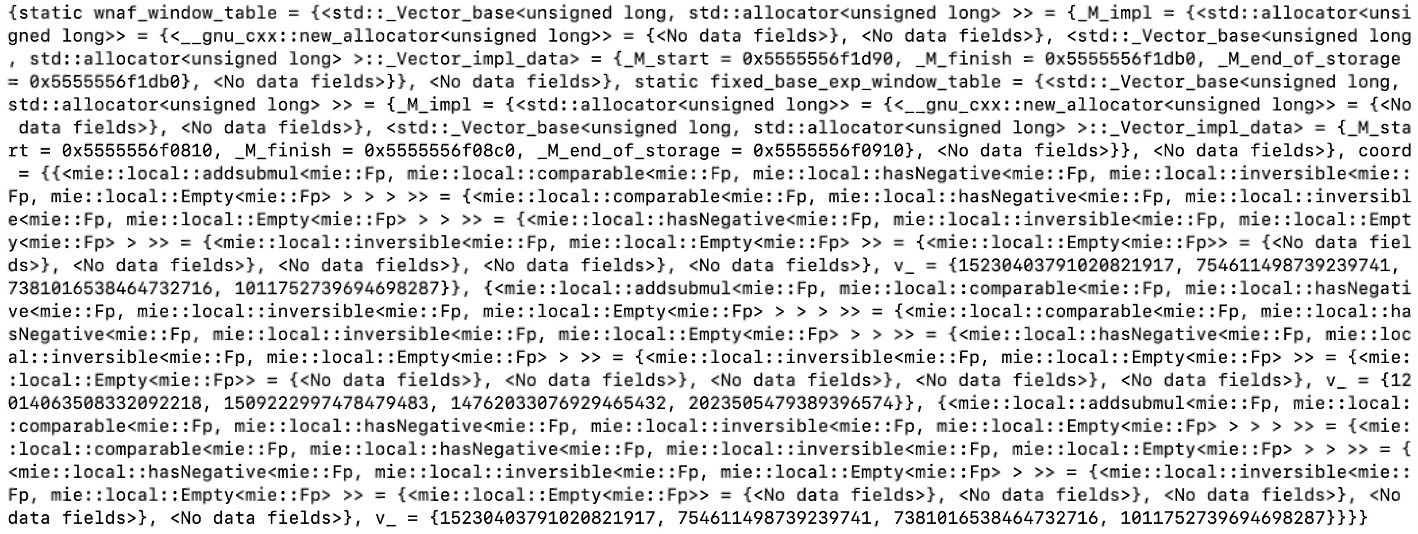
\includegraphics[width=\textwidth]{ch-snarkprobe/figure/prettyprint-a.jpg}
  \caption{Content without PrettyPrint in \libsnark}
  \label{subfig:snarkprobe-prettyprint_a}
\end{subfigure}
\par\vspace{10pt}
\begin{subfigure}{0.9\textwidth}
  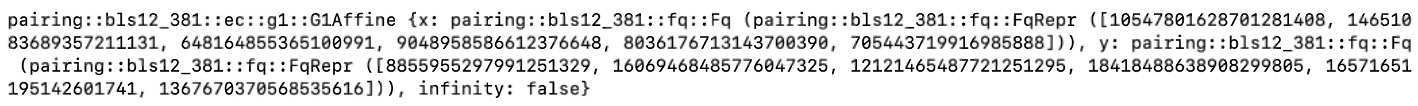
\includegraphics[width=\textwidth]{ch-snarkprobe/figure/prettyprint-b.jpg}
  \caption{Content without PrettyPrint in \bellman}
  \label{subfig:snarkprobe-prettyprint_b}
\end{subfigure}
\par\vspace{10pt}
\begin{subfigure}{0.9\textwidth}
  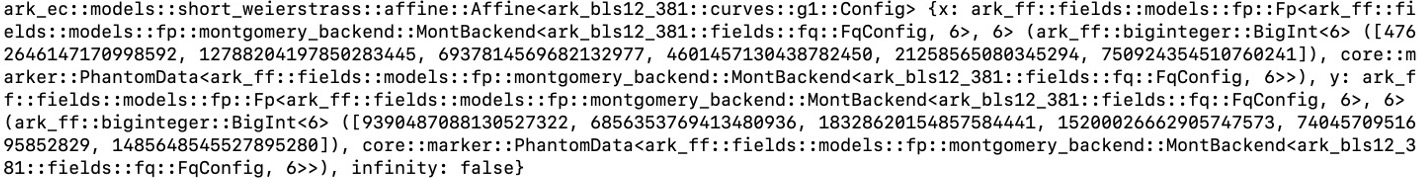
\includegraphics[width=\textwidth]{ch-snarkprobe/figure/prettyprint-c.jpg}
  \caption{Content without PrettyPrint in \arkworks}
  \label{subfig:snarkprobe-prettyprint_c}
\end{subfigure}
\par\vspace{10pt}
\begin{subfigure}{0.9\textwidth}
  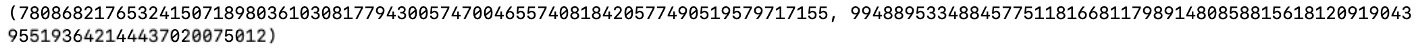
\includegraphics[width=\textwidth]{ch-snarkprobe/figure/prettyprint-d.jpg}
  \caption{Content with PrettyPrint in any library}
  \label{subfig:snarkprobe-prettyprint_d}
\end{subfigure}
\caption{Content of variable type G1}
\label{fig:snarkprobe-prettyprint}
\end{figure}



\parheadit{\valueextractor.}
The \valueextractor extracts all variables defined in the ideal value file using GDB and PrettyPrint.  As the ideal value file contains the line number where each variable is assigned, the \valueextractor can automatically set up a breakpoint for each variable immediately after its assignment. Then, when the input program reaches this, the \valueextractor uses PrettyPrint to save the variable's formatted value. %The program will continually run until all GDB breakpoints have been hit and all variables' values have been saved.

\parheadit{\valuechecker.}
%\label{secsec:snarkprobe-impvaluechecker}
We developed the \valuechecker for \pinocchio by following \cite{parno2013pinocchio} and \cite{ben2014succinct} and \groth16 by \cite{groth2016size} and \cite{nitulescu2020zk}. To help ensure accurate re-evaluation of the protocol calculations, the \valuechecker uses exactly the same variable names as the original papers, and we follow the protocol description exactly, without any optimizations, to avoid introducing mistakes.

\parheadit{ECC Libraries.} We use two well-tested elliptic curve libraries to demonstrate diversity and flexibility.
py\_ecc \cite{pyecc}, developed by Ethereum in Python, supports both the BN128 and BLS12-381 curves. CIRCL \cite{circl}, developed by Cloudflare in Go, supports BLS12-381.  Since it is written in Go, we developed the necessary APIs so that our Python-based \valuechecker can access the functions. If users would like to test a new zkSNARK library using a curve that py\_ecc or CIRCL do not support, they can easily plug it into the \valuechecker in this same manner.

%%%%%%%%%%


\subsubsection*{\underline{\SnarkFuzzer: \valuemonitor}}
\label{subsec:snarkprobe-value-monitor}

\textbf{Goals: } \emph{The \valuemonitor detects any unexpected value changes after the extraction of initial variable values from the source program.}

\parhead{Design.}%
While the \valuemodel extracts all necessary variables' values at the location where the variables are first assigned, and we also need to check if there is a value change after the model extracts these values to ensure consistency between the library and the \valuechecker. The \valuemonitor can also detect any unexpected side effects caused by the library or dependent functions due to incorrect implementation, out of memory, or other unexpected errors.

\parhead{Implementation.}%
GDB watch allows \SnarkFuzzer to monitor value changes in a debugging session with four CPU debug registers called hardware watchpoints. A hardware watchpoint is very efficient, but it does not support larger data structures given the limited debug registers. Software watchpoints will be automatically applied if GDB tries to setup a watchpoint for a variable that cannot be handled by a hardware watchpoint. Unlike hardware watchpoints, software watchpoints are extremely slow, and watching dozens of variables may require unacceptable processing time. For example, using GDB software watch for a single variable \texttt{A\_query} in \libsnark takes more than 30 minutes.

Therefore, we instead used Valgrind, a dynamic analysis tool that analyzes a program to automatically detect memory management and threading bugs. Valgrind has a gdbserver to simulate traditional GDB hardware watchpoints. Simulation still takes longer than pure GDB hardware watchpoints, but the hardware watchpoint simulation is much faster than GDB software watchpoints. Meanwhile, Valgrind hardware watchpoint simulation does not have any limitation on the number and length of variables, so Valgrind can be used for any zkSNARK source program and libraries with complex data structures.